%& /home/ignazio/.config/TikzEdtWForms/TikzEdtWForms/0.2.1.0/temp_header
\begin{document}
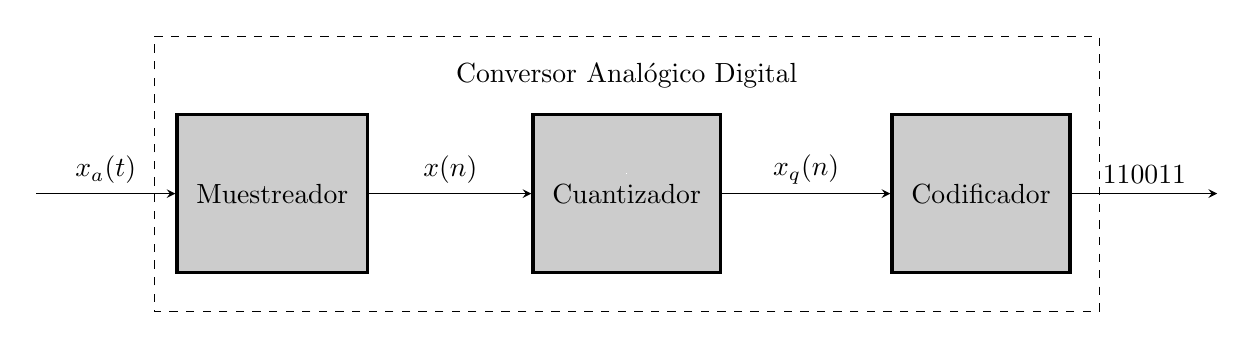
\begin{tikzpicture}
\tikzstyle{box} = [draw,inner sep=7,minimum size=57,line 
						   width=1, very thick, draw=black, fill=black!20]
\tikzstyle{invisible} = [outer sep=0,inner sep=0,minimum size=0]
\tikzstyle{stealth} = [-stealth]
\node [box] (v1) at (-1,0.5) {Muestreador};
\node [box] (v2) at (3.5,0.5) {Cuantizador};
\node [box] (v3) at (8,0.5) {Codificador};
\draw [stealth] (v1) edge node [anchor=south] {$x(n)$} (v2);
\draw [stealth] (v2) edge node [anchor=south] {$x_q(n)$} (v3);
\node [invisible] (v4) at (-4,0.5) {};
\draw [stealth] (v4) edge node [anchor=south] {$x_a(t)$} (v1);
\node [invisible] (v5) at (11,0.5) {};
\draw [stealth] (v3) edge node [anchor=south] {$110011$} (v5);
\draw [dashed] (-2.5,2.5) node [invisible] (v6) {} -- (9.5,2.5) node [invisible] {} -- 
	  (9.5,-1) node [invisible] {} -- (-2.5,-1) node [invisible] {} -- (v6);
\node [invisible] at (3.5,2) {Conversor Analógico Digital};

\usetikzlibrary{calc}
\pgftransformreset
\node[inner sep=0pt,outer sep=0pt,minimum size=0pt,line width=0pt,text width=0pt,text height=0pt] at (current bounding box) {};
%add border to avoid cropping by pdflibnet
\foreach \border in {0.1}
  \useasboundingbox (current bounding box.south west)+(-\border,-\border) rectangle (current bounding box.north east)+(\border,\border);
\newwrite\metadatafile
\immediate\openout\metadatafile=\jobname_BB.txt
\path
  let
    \p1=(current bounding box.south west),
    \p2=(current bounding box.north east)
  in
  node[inner sep=0pt,outer sep=0pt,minimum size=0pt,line width=0pt,text width=0pt,text height=0pt,draw=white] at (current bounding box) {
\immediate\write\metadatafile{\p1,\p2}
};
\immediate\closeout\metadatafile
\end{tikzpicture}

\end{document}
